\documentclass[twoside]{book}

% Packages required by doxygen
\usepackage{calc}
\usepackage{doxygen}
\usepackage{graphicx}
\usepackage[utf8]{inputenc}
\usepackage{makeidx}
\usepackage{multicol}
\usepackage{multirow}
\usepackage{textcomp}
\usepackage[table]{xcolor}

% Font selection
\usepackage[T1]{fontenc}
\usepackage{mathptmx}
\usepackage[scaled=.90]{helvet}
\usepackage{courier}
\usepackage{amssymb}
\usepackage{sectsty}
\renewcommand{\familydefault}{\sfdefault}
\allsectionsfont{%
  \fontseries{bc}\selectfont%
  \color{darkgray}%
}
\renewcommand{\DoxyLabelFont}{%
  \fontseries{bc}\selectfont%
  \color{darkgray}%
}

% Page & text layout
\usepackage{geometry}
\geometry{%
  a4paper,%
  top=2.5cm,%
  bottom=2.5cm,%
  left=2.5cm,%
  right=2.5cm%
}
\tolerance=750
\hfuzz=15pt
\hbadness=750
\setlength{\emergencystretch}{15pt}
\setlength{\parindent}{0cm}
\setlength{\parskip}{0.2cm}
\makeatletter
\renewcommand{\paragraph}{%
  \@startsection{paragraph}{4}{0ex}{-1.0ex}{1.0ex}{%
    \normalfont\normalsize\bfseries\SS@parafont%
  }%
}
\renewcommand{\subparagraph}{%
  \@startsection{subparagraph}{5}{0ex}{-1.0ex}{1.0ex}{%
    \normalfont\normalsize\bfseries\SS@subparafont%
  }%
}
\makeatother

% Headers & footers
\usepackage{fancyhdr}
\pagestyle{fancyplain}
\fancyhead[LE]{\fancyplain{}{\bfseries\thepage}}
\fancyhead[CE]{\fancyplain{}{}}
\fancyhead[RE]{\fancyplain{}{\bfseries\leftmark}}
\fancyhead[LO]{\fancyplain{}{\bfseries\rightmark}}
\fancyhead[CO]{\fancyplain{}{}}
\fancyhead[RO]{\fancyplain{}{\bfseries\thepage}}
\fancyfoot[LE]{\fancyplain{}{}}
\fancyfoot[CE]{\fancyplain{}{}}
\fancyfoot[RE]{\fancyplain{}{\bfseries\scriptsize Generated on Tue Jun 24 2014 22\-:40\-:11 for B\-E\-N the Robot by Doxygen }}
\fancyfoot[LO]{\fancyplain{}{\bfseries\scriptsize Generated on Tue Jun 24 2014 22\-:40\-:11 for B\-E\-N the Robot by Doxygen }}
\fancyfoot[CO]{\fancyplain{}{}}
\fancyfoot[RO]{\fancyplain{}{}}
\renewcommand{\footrulewidth}{0.4pt}
\renewcommand{\chaptermark}[1]{%
  \markboth{#1}{}%
}
\renewcommand{\sectionmark}[1]{%
  \markright{\thesection\ #1}%
}

% Indices & bibliography
\usepackage{natbib}
\usepackage[titles]{tocloft}
\setcounter{tocdepth}{3}
\setcounter{secnumdepth}{5}
\makeindex

% Hyperlinks (required, but should be loaded last)
\usepackage{ifpdf}
\ifpdf
  \usepackage[pdftex,pagebackref=true]{hyperref}
\else
  \usepackage[ps2pdf,pagebackref=true]{hyperref}
\fi
\hypersetup{%
  colorlinks=true,%
  linkcolor=blue,%
  citecolor=blue,%
  unicode%
}

% Custom commands
\newcommand{\clearemptydoublepage}{%
  \newpage{\pagestyle{empty}\cleardoublepage}%
}


%===== C O N T E N T S =====

\begin{document}

% Titlepage & ToC
\hypersetup{pageanchor=false}
\pagenumbering{roman}
\begin{titlepage}
\vspace*{7cm}
\begin{center}%
{\Large B\-E\-N the Robot \\[1ex]\large 0.\-1 }\\
\vspace*{1cm}
{\large Generated by Doxygen 1.8.6}\\
\vspace*{0.5cm}
{\small Tue Jun 24 2014 22:40:11}\\
\end{center}
\end{titlepage}
\clearemptydoublepage
\tableofcontents
\clearemptydoublepage
\pagenumbering{arabic}
\hypersetup{pageanchor=true}

%--- Begin generated contents ---
\chapter{Main Page}
\label{index}\hypertarget{index}{}The code controlling the Raspberry Pi on my robot, B\-E\-N (Bright Enough to Navigate)

\subsection*{ping sensor}


\begin{DoxyItemize}
\item stores trigger pin number
\item stores echo pin number
\item gives distance
\end{DoxyItemize}

\subsection*{world}


\begin{DoxyItemize}
\item 2d linked-\/list of squares
\end{DoxyItemize}

\subsection*{square}


\begin{DoxyItemize}
\item number of times scanned
\item number of times object found here
\item linked list of coordinates that this square has been scanned from
\item x coordinate
\item y coordinate
\end{DoxyItemize}

\subsection*{mysql}


\begin{DoxyItemize}
\item stores maps from each run
\end{DoxyItemize}

\subsection*{threads}

in order of priority


\begin{DoxyItemize}
\item 1 thread for bump sensors
\item 1 main thread
\item 1 thread for movement
\item 4 threads for ping sensors
\begin{DoxyItemize}
\item they will alternate between sensors
\end{DoxyItemize}
\item 1 thread for processing sensor data
\item 1 thread for finding best path
\item 1 thread for machine learning 
\end{DoxyItemize}
\chapter{Namespace Index}
\section{Namespace List}
Here is a list of all documented namespaces with brief descriptions\-:\begin{DoxyCompactList}
\item\contentsline{section}{\hyperlink{namespaceutils}{utils} }{\pageref{namespaceutils}}{}
\end{DoxyCompactList}

\chapter{Hierarchical Index}
\section{Class Hierarchy}
This inheritance list is sorted roughly, but not completely, alphabetically\-:\begin{DoxyCompactList}
\item \contentsline{section}{Main}{\pageref{classMain}}{}
\item \contentsline{section}{Ping}{\pageref{classPing}}{}
\item Bug\begin{DoxyCompactList}
\item \contentsline{section}{Path\-Bug}{\pageref{classPathBug}}{}
\begin{DoxyCompactList}
\item \contentsline{section}{A\-Star\-Bug}{\pageref{classAStarBug}}{}
\end{DoxyCompactList}
\end{DoxyCompactList}
\end{DoxyCompactList}

\chapter{Class Index}
\section{Class List}
Here are the classes, structs, unions and interfaces with brief descriptions\-:\begin{DoxyCompactList}
\item\contentsline{section}{\hyperlink{classAStarBug}{A\-Star\-Bug} }{\pageref{classAStarBug}}{}
\item\contentsline{section}{\hyperlink{classMain}{Main} }{\pageref{classMain}}{}
\item\contentsline{section}{\hyperlink{classPathBug}{Path\-Bug} }{\pageref{classPathBug}}{}
\item\contentsline{section}{\hyperlink{classPing}{Ping} }{\pageref{classPing}}{}
\end{DoxyCompactList}

\chapter{File Index}
\section{File List}
Here is a list of all documented files with brief descriptions\-:\begin{DoxyCompactList}
\item\contentsline{section}{\hyperlink{base_8h}{base.\-h} }{\pageref{base_8h}}{}
\item\contentsline{section}{\hyperlink{main_8cpp}{main.\-cpp} }{\pageref{main_8cpp}}{}
\item\contentsline{section}{{\bfseries main.\-h} }{\pageref{main_8h}}{}
\item\contentsline{section}{\hyperlink{ping_8h}{ping.\-h} }{\pageref{ping_8h}}{}
\item\contentsline{section}{{\bfseries utils.\-h} }{\pageref{utils_8h}}{}
\end{DoxyCompactList}

\chapter{Namespace Documentation}
\hypertarget{namespaceutils}{\section{utils Namespace Reference}
\label{namespaceutils}\index{utils@{utils}}
}
\subsection*{Functions}
\begin{DoxyCompactItemize}
\item 
long \hyperlink{namespaceutils_a119f267acdf7deb4a7fd994c171929d9}{pulse\-In} (int pin, int level, int timeout)
\end{DoxyCompactItemize}


\subsection{Detailed Description}
Utilities namespace contains useful functions that aren't really associated with anything else, such as Arduino-\/esque functions not included in Wiring\-Pi 

\subsection{Function Documentation}
\hypertarget{namespaceutils_a119f267acdf7deb4a7fd994c171929d9}{\index{utils@{utils}!pulse\-In@{pulse\-In}}
\index{pulse\-In@{pulse\-In}!utils@{utils}}
\subsubsection[{pulse\-In}]{\setlength{\rightskip}{0pt plus 5cm}long utils\-::pulse\-In (
\begin{DoxyParamCaption}
\item[{int}]{pin, }
\item[{int}]{level, }
\item[{int}]{timeout}
\end{DoxyParamCaption}
)}}\label{namespaceutils_a119f267acdf7deb4a7fd994c171929d9}
Calculates the length of a pulse on a pin 
\begin{DoxyParams}{Parameters}
{\em pin} & the G\-P\-I\-O pin number to watch \\
\hline
{\em level} & what level of pulse to look for. Either H\-I\-G\-H or L\-O\-W \\
\hline
{\em timeout} & the maximum length of a pulse \\
\hline
\end{DoxyParams}
\begin{DoxyReturn}{Returns}
the length of the pulse in microseconds 
\end{DoxyReturn}

\chapter{Class Documentation}
\hypertarget{classAStarBug}{\section{A\-Star\-Bug Class Reference}
\label{classAStarBug}\index{A\-Star\-Bug@{A\-Star\-Bug}}
}
Inheritance diagram for A\-Star\-Bug\-:\begin{figure}[H]
\begin{center}
\leavevmode
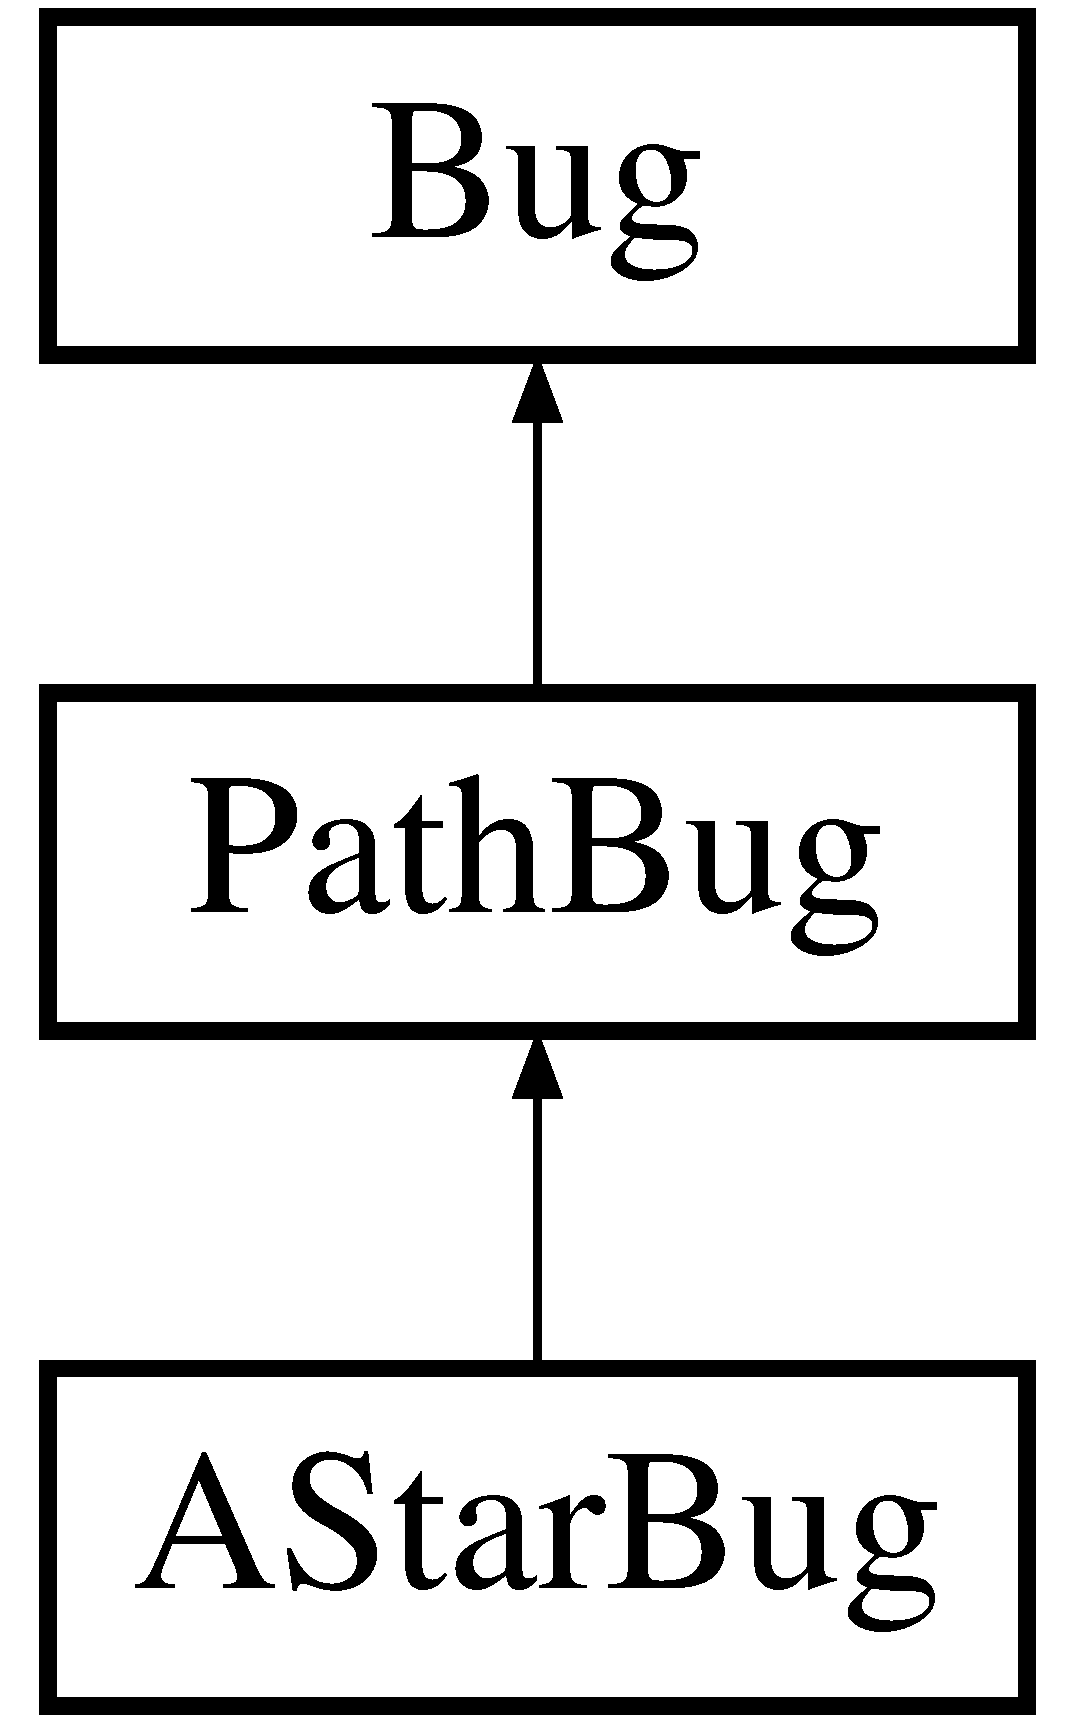
\includegraphics[height=3.000000cm]{classAStarBug}
\end{center}
\end{figure}
\subsection*{Public Member Functions}
\begin{DoxyCompactItemize}
\item 
\hypertarget{classAStarBug_adce292fcb395242f566e6b194d6385ac}{{\bfseries A\-Star\-Bug} (Location destination)}\label{classAStarBug_adce292fcb395242f566e6b194d6385ac}

\end{DoxyCompactItemize}
\subsection*{Protected Member Functions}
\begin{DoxyCompactItemize}
\item 
\hypertarget{classAStarBug_a3a806b7fad5707103c5ad3fb3895a5b3}{int\mbox{[}$\,$\mbox{]} {\bfseries get\-Path} (Location destination)}\label{classAStarBug_a3a806b7fad5707103c5ad3fb3895a5b3}

\end{DoxyCompactItemize}


The documentation for this class was generated from the following file\-:\begin{DoxyCompactItemize}
\item 
A\-Star\-Bug.\-java\end{DoxyCompactItemize}

\hypertarget{classMain}{\section{Main Class Reference}
\label{classMain}\index{Main@{Main}}
}
\subsection*{Static Public Member Functions}
\begin{DoxyCompactItemize}
\item 
\hypertarget{classMain_a8a5d0f827edddff706cc0e6740d0579a}{static void {\bfseries main} (String\mbox{[}$\,$\mbox{]} args)}\label{classMain_a8a5d0f827edddff706cc0e6740d0579a}

\end{DoxyCompactItemize}


The documentation for this class was generated from the following file\-:\begin{DoxyCompactItemize}
\item 
Main.\-java\end{DoxyCompactItemize}

\hypertarget{classPathBug}{\section{Path\-Bug Class Reference}
\label{classPathBug}\index{Path\-Bug@{Path\-Bug}}
}
Inheritance diagram for Path\-Bug\-:\begin{figure}[H]
\begin{center}
\leavevmode
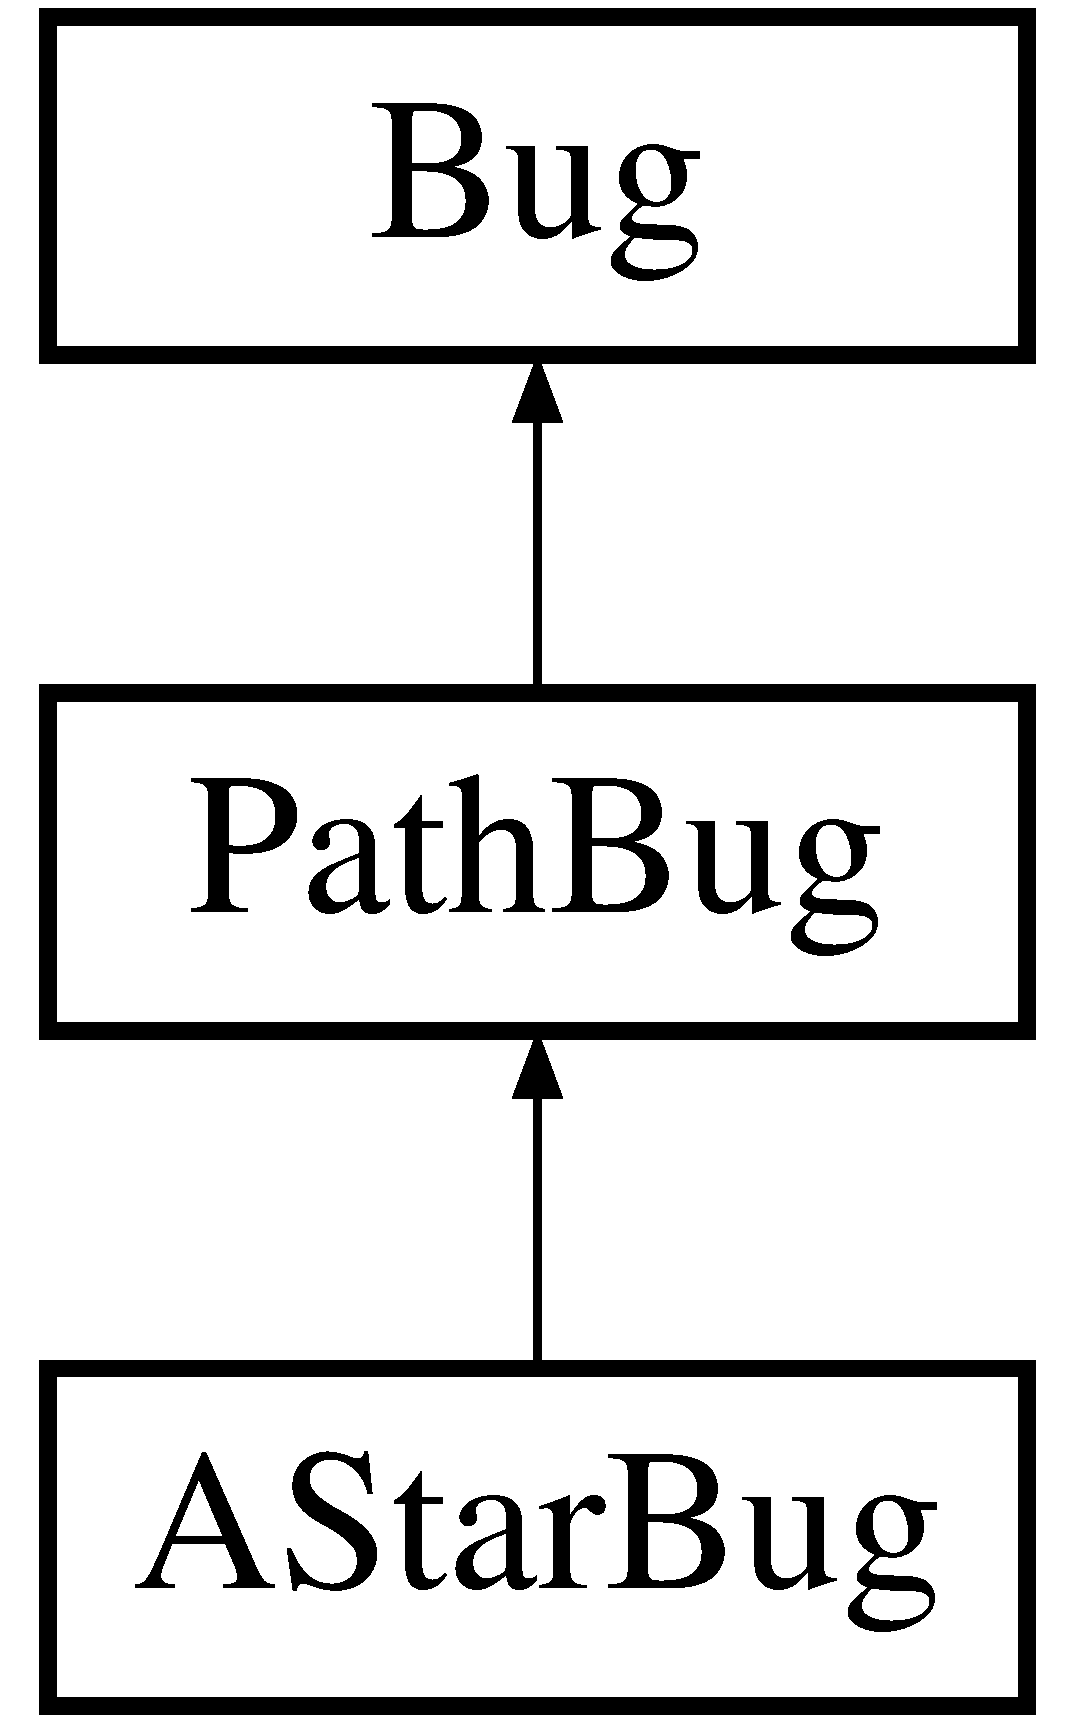
\includegraphics[height=3.000000cm]{classPathBug}
\end{center}
\end{figure}
\subsection*{Public Member Functions}
\begin{DoxyCompactItemize}
\item 
\hypertarget{classPathBug_a26ac068b0f789add7c3d0f32ec8c0b98}{{\bfseries Path\-Bug} (Location destination)}\label{classPathBug_a26ac068b0f789add7c3d0f32ec8c0b98}

\item 
\hypertarget{classPathBug_a5a0980aac2f4ba3eb97ade9de758d517}{void {\bfseries turn} ()}\label{classPathBug_a5a0980aac2f4ba3eb97ade9de758d517}

\item 
\hypertarget{classPathBug_a1a6abdca2f1c4892320fbca8a0a8b5b7}{void {\bfseries act} ()}\label{classPathBug_a1a6abdca2f1c4892320fbca8a0a8b5b7}

\end{DoxyCompactItemize}
\subsection*{Protected Member Functions}
\begin{DoxyCompactItemize}
\item 
\hypertarget{classPathBug_a75ceded2dc68b195d018417553f7a8d8}{abstract int\mbox{[}$\,$\mbox{]} {\bfseries get\-Path} (Location destination)}\label{classPathBug_a75ceded2dc68b195d018417553f7a8d8}

\end{DoxyCompactItemize}


The documentation for this class was generated from the following file\-:\begin{DoxyCompactItemize}
\item 
Path\-Bug.\-java\end{DoxyCompactItemize}

\hypertarget{classPing}{\section{Ping Class Reference}
\label{classPing}\index{Ping@{Ping}}
}


{\ttfamily \#include $<$ping.\-h$>$}

\subsection*{Public Member Functions}
\begin{DoxyCompactItemize}
\item 
\hyperlink{classPing_ac8699f06de93bae019b5c10eb4d9f07e}{Ping} (int temp\-Trigger\-Pin, int temp\-Echo\-Pin)
\item 
void \hyperlink{classPing_a60a84a4161b40e9fb7f82cabf6a948fc}{init} ()
\item 
long \hyperlink{classPing_a683f58ccb6bd5ef4c8ee82f2cf0a1652}{get\-Inches} ()
\item 
long \hyperlink{classPing_aae84b003ab46fbbc9ac591df3ab61e89}{get\-Centimeters} ()
\end{DoxyCompactItemize}


\subsection{Detailed Description}
Provides an interface to use the ping sensor 

\subsection{Constructor \& Destructor Documentation}
\hypertarget{classPing_ac8699f06de93bae019b5c10eb4d9f07e}{\index{Ping@{Ping}!Ping@{Ping}}
\index{Ping@{Ping}!Ping@{Ping}}
\subsubsection[{Ping}]{\setlength{\rightskip}{0pt plus 5cm}Ping\-::\-Ping (
\begin{DoxyParamCaption}
\item[{int}]{temp\-Trigger\-Pin, }
\item[{int}]{temp\-Echo\-Pin}
\end{DoxyParamCaption}
)}}\label{classPing_ac8699f06de93bae019b5c10eb4d9f07e}
Initializes pin numbers 
\begin{DoxyParams}{Parameters}
{\em temp\-Trigger\-Pin} & the pin number for the trigger pin \\
\hline
{\em temp\-Echo\-Pin} & the pin number for the echo pin \\
\hline
\end{DoxyParams}


\subsection{Member Function Documentation}
\hypertarget{classPing_aae84b003ab46fbbc9ac591df3ab61e89}{\index{Ping@{Ping}!get\-Centimeters@{get\-Centimeters}}
\index{get\-Centimeters@{get\-Centimeters}!Ping@{Ping}}
\subsubsection[{get\-Centimeters}]{\setlength{\rightskip}{0pt plus 5cm}long Ping\-::get\-Centimeters (
\begin{DoxyParamCaption}
{}
\end{DoxyParamCaption}
)}}\label{classPing_aae84b003ab46fbbc9ac591df3ab61e89}
Uses the ping sensor to takes a reading and returns the distance in centimeters \begin{DoxyReturn}{Returns}
the distance in centimeters 
\end{DoxyReturn}
\hypertarget{classPing_a683f58ccb6bd5ef4c8ee82f2cf0a1652}{\index{Ping@{Ping}!get\-Inches@{get\-Inches}}
\index{get\-Inches@{get\-Inches}!Ping@{Ping}}
\subsubsection[{get\-Inches}]{\setlength{\rightskip}{0pt plus 5cm}long Ping\-::get\-Inches (
\begin{DoxyParamCaption}
{}
\end{DoxyParamCaption}
)}}\label{classPing_a683f58ccb6bd5ef4c8ee82f2cf0a1652}
Uses the ping sensor to takes a reading and returns the distance in inches \begin{DoxyReturn}{Returns}
the distance in inches 
\end{DoxyReturn}
\hypertarget{classPing_a60a84a4161b40e9fb7f82cabf6a948fc}{\index{Ping@{Ping}!init@{init}}
\index{init@{init}!Ping@{Ping}}
\subsubsection[{init}]{\setlength{\rightskip}{0pt plus 5cm}void Ping\-::init (
\begin{DoxyParamCaption}
{}
\end{DoxyParamCaption}
)}}\label{classPing_a60a84a4161b40e9fb7f82cabf6a948fc}
Initilizes the pins to be ready to be used. Must be called before any other function and in \hyperlink{base_8h_a4fc01d736fe50cf5b977f755b675f11d}{setup()}. 

The documentation for this class was generated from the following files\-:\begin{DoxyCompactItemize}
\item 
\hyperlink{ping_8h}{ping.\-h}\item 
ping.\-cpp\end{DoxyCompactItemize}

\chapter{File Documentation}
\hypertarget{base_8h}{\section{base.\-h File Reference}
\label{base_8h}\index{base.\-h@{base.\-h}}
}
\subsection*{Functions}
\begin{DoxyCompactItemize}
\item 
void \hyperlink{base_8h_a4fc01d736fe50cf5b977f755b675f11d}{setup} ()
\item 
void \hyperlink{base_8h_afe461d27b9c48d5921c00d521181f12f}{loop} ()
\item 
void \hyperlink{base_8h_a4b66d5e31b5dc18b314c8a68163263bd}{cleanup} ()
\item 
int \hyperlink{base_8h_ae66f6b31b5ad750f1fe042a706a4e3d4}{main} ()
\end{DoxyCompactItemize}


\subsection{Function Documentation}
\hypertarget{base_8h_a4b66d5e31b5dc18b314c8a68163263bd}{\index{base.\-h@{base.\-h}!cleanup@{cleanup}}
\index{cleanup@{cleanup}!base.h@{base.\-h}}
\subsubsection[{cleanup}]{\setlength{\rightskip}{0pt plus 5cm}void cleanup (
\begin{DoxyParamCaption}
{}
\end{DoxyParamCaption}
)}}\label{base_8h_a4b66d5e31b5dc18b314c8a68163263bd}
called at program end (or interrupt) to clean up any classes that need cleaning up and save any data that need saving \hypertarget{base_8h_afe461d27b9c48d5921c00d521181f12f}{\index{base.\-h@{base.\-h}!loop@{loop}}
\index{loop@{loop}!base.h@{base.\-h}}
\subsubsection[{loop}]{\setlength{\rightskip}{0pt plus 5cm}void loop (
\begin{DoxyParamCaption}
{}
\end{DoxyParamCaption}
)}}\label{base_8h_afe461d27b9c48d5921c00d521181f12f}
called at program end (or interrupt) to clean up any classes that need cleaning up and save any data that need saving \hypertarget{base_8h_ae66f6b31b5ad750f1fe042a706a4e3d4}{\index{base.\-h@{base.\-h}!main@{main}}
\index{main@{main}!base.h@{base.\-h}}
\subsubsection[{main}]{\setlength{\rightskip}{0pt plus 5cm}int main (
\begin{DoxyParamCaption}
{}
\end{DoxyParamCaption}
)}}\label{base_8h_ae66f6b31b5ad750f1fe042a706a4e3d4}
main function, should not be touched. Instead define \hyperlink{base_8h_a4fc01d736fe50cf5b977f755b675f11d}{setup()}, \hyperlink{base_8h_afe461d27b9c48d5921c00d521181f12f}{loop()} and \hyperlink{base_8h_a4b66d5e31b5dc18b314c8a68163263bd}{cleanup()}. provides safe exiting and G\-P\-I\-O access \hypertarget{base_8h_a4fc01d736fe50cf5b977f755b675f11d}{\index{base.\-h@{base.\-h}!setup@{setup}}
\index{setup@{setup}!base.h@{base.\-h}}
\subsubsection[{setup}]{\setlength{\rightskip}{0pt plus 5cm}void setup (
\begin{DoxyParamCaption}
{}
\end{DoxyParamCaption}
)}}\label{base_8h_a4fc01d736fe50cf5b977f755b675f11d}
called at beginning of execution to initilize everything properly 
\hypertarget{main_8cpp}{\section{main.\-cpp File Reference}
\label{main_8cpp}\index{main.\-cpp@{main.\-cpp}}
}
{\ttfamily \#include \char`\"{}main.\-h\char`\"{}}\\*
{\ttfamily \#include \char`\"{}ping.\-h\char`\"{}}\\*
{\ttfamily \#include \char`\"{}base.\-h\char`\"{}}\\*
{\ttfamily \#include $<$iostream$>$}\\*
{\ttfamily \#include $<$wiring\-Pi.\-h$>$}\\*
\subsection*{Functions}
\begin{DoxyCompactItemize}
\item 
void \hyperlink{main_8cpp_a4fc01d736fe50cf5b977f755b675f11d}{setup} ()
\item 
void \hyperlink{main_8cpp_afe461d27b9c48d5921c00d521181f12f}{loop} ()
\item 
void \hyperlink{main_8cpp_a4b66d5e31b5dc18b314c8a68163263bd}{cleanup} ()
\end{DoxyCompactItemize}
\subsection*{Variables}
\begin{DoxyCompactItemize}
\item 
\hypertarget{main_8cpp_a991b200891f080644fadd7f036dc8ca7}{\hyperlink{classPing}{Ping} {\bfseries sensor} (24, 25)}\label{main_8cpp_a991b200891f080644fadd7f036dc8ca7}

\end{DoxyCompactItemize}


\subsection{Function Documentation}
\hypertarget{main_8cpp_a4b66d5e31b5dc18b314c8a68163263bd}{\index{main.\-cpp@{main.\-cpp}!cleanup@{cleanup}}
\index{cleanup@{cleanup}!main.cpp@{main.\-cpp}}
\subsubsection[{cleanup}]{\setlength{\rightskip}{0pt plus 5cm}void cleanup (
\begin{DoxyParamCaption}
{}
\end{DoxyParamCaption}
)}}\label{main_8cpp_a4b66d5e31b5dc18b314c8a68163263bd}
called at program end (or interrupt) to clean up any classes that need cleaning up and save any data that need saving \hypertarget{main_8cpp_afe461d27b9c48d5921c00d521181f12f}{\index{main.\-cpp@{main.\-cpp}!loop@{loop}}
\index{loop@{loop}!main.cpp@{main.\-cpp}}
\subsubsection[{loop}]{\setlength{\rightskip}{0pt plus 5cm}void loop (
\begin{DoxyParamCaption}
{}
\end{DoxyParamCaption}
)}}\label{main_8cpp_afe461d27b9c48d5921c00d521181f12f}
called at program end (or interrupt) to clean up any classes that need cleaning up and save any data that need saving \hypertarget{main_8cpp_a4fc01d736fe50cf5b977f755b675f11d}{\index{main.\-cpp@{main.\-cpp}!setup@{setup}}
\index{setup@{setup}!main.cpp@{main.\-cpp}}
\subsubsection[{setup}]{\setlength{\rightskip}{0pt plus 5cm}void setup (
\begin{DoxyParamCaption}
{}
\end{DoxyParamCaption}
)}}\label{main_8cpp_a4fc01d736fe50cf5b977f755b675f11d}
called at beginning of execution to initilize everything properly 
\hypertarget{ping_8h}{\section{ping.\-h File Reference}
\label{ping_8h}\index{ping.\-h@{ping.\-h}}
}
\subsection*{Classes}
\begin{DoxyCompactItemize}
\item 
class \hyperlink{classPing}{Ping}
\end{DoxyCompactItemize}

%--- End generated contents ---

% Index
\newpage
\phantomsection
\addcontentsline{toc}{chapter}{Index}
\printindex

\end{document}
